\chapter{Metodologia}
\label{chap:metodologia}

Este capítulo apresenta o método experimental para avaliação comparativa 
de algoritmos de agregação robusta em Aprendizado Federado (\gls{fl}) sob 
cenários adversariais, com ênfase em heterogeneidade de dados (\gls{noniid}) 
e ataques de \textit{model poisoning}. A pesquisa adota abordagem 
quantitativa e experimental, com replicação estatística e análise de 
inferência.

\section{Etapas do Desenvolvimento Experimental}

\subsection{Etapa 1: Visão Geral e Preparação}

O desenho experimental segue o paradigma fatorial completo, 
permitindo análise de efeitos principais e interações entre fatores 
\cite{Montgomery2017}. O objetivo é testar a hipótese de que agregadores 
robustos mantêm desempenho superior ao \textit{baseline} (FedAvg) sob 
múltiplos tipos e intensidades de ataques, com generalização verificada em domínios de dados distintos.

O \textit{pipeline} computacional compreende: (i) preparação de dados com particionamento controlado; (ii) simulação federada restrita aos cenários delineados; (iii) variação sistemática da intensidade adversarial e \gls{noniid}; e (iv) coleta de métricas globais e análise estatística.

\subsection{Etapa 2: Conjuntos de Dados e Pré-processamento}

\subsection{MNIST}
Dataset \textit{benchmark} de dígitos manuscritos \cite{LeCun1998}, com 
60.000 imagens de treinamento e 10.000 de teste (28$\times$28 pixels, 
10 classes). Utilizado para avaliação principal e espaço de testes exaustivo, devido à adoção 
consensual na literatura de \gls{fl} robusto.

\subsection{Fashion-MNIST}
Dataset de imagens de vestuário \cite{Xiao2017}, com mesmas dimensões 
do MNIST mas maior complexidade visual e fronteiras de decisão mais 
nuançadas. Utilizado seletivamente para validação de generalização de domínio em cenários de ataques persistentes e de alta eficácia
\cite{Kairouz2021}.

\subsection{Pré-processamento}
Os dados sofreram normalização exclusiva para [0,1] via vetorização de características (\texttt{ToTensor()}), sem a incidência de \textit{data augmentation} para preservar estrita comparabilidade paramétrica com trabalhos anteriores.

\subsection{Etapa 3: Arquitetura da Federação e Hiperparâmetros}

A estrutura cliente-servidor foi modelada segundo o comportamento nativo de agregação paralela:
\begin{itemize}
    \item \textbf{Clientes}: $N = 100$ total simulados;
    \item \textbf{Participação por Rodada}: $C = 0.1$ (10 clientes engajados ativamente, amostragem aleatória uniforme, sem reposição);
    \item \textbf{Rodadas Globais}: $R = 200$;
    \item \textbf{Épocas locais ($E$)}: restritas a $1$ atualização completa por nó (isolando o tempo de divergência associado a longos treinamentos desgovernados, favorecendo o mapeamento isolado da robustez do agregador) \cite{Chen2023};
    \item \textbf{Otimizador local}: SGD ($\eta = 0.01$, momentum $= 0.9$);
    \item \textbf{\textit{Batch} local}: $B = 32$.
\end{itemize}

\subsection{Etapa 4: Modelagem da Heterogeneidade (Non-IID)}

Empregou-se o modelo de partição assimétrica Dirichlet \cite{Hsu2019}:
\begin{equation}
    \mathbf{p}_k \sim \text{Dir}(\alpha \cdot \mathbf{1})
\end{equation}

onde $\mathbf{p}_k$ denota a distribuição das classes de saída latentes no cliente $k$.
Foram gerados cenários com $\alpha \in \{0.1, 0.5, 1.0\}$. Assim, $\alpha=0.1$ impõem alta heterogeneidade (dados enviesados; 1 ou 2 classes principais possuídas por ator), $\alpha=0.5$ induz dispersão de grau médio-alto e $\alpha=1.0$ representa limite estendido e leve (desvios mais brandos da normalidade IID).

\section{Arquitetura do Modelo Local e Ameaça}

Todos os agentes, benignos ou maliciosos, treinam através de uma topologia convolucional unificada: duas camadas convolucionais \textit{2D} combinadas com ativação ReLU e funções de \textit{Max-Pooling}, desaguando numa malha densa de classificação cruzada de entropia, somatizando em cerca de 3.2M parâmetros de arquitetura fixa.

\subsection{O Atacante (\textit{Model Poisoning})}
A atuação comprometedora adotou caráter de falhas operacionais hostis (\textbf{ataques não direcionados}): operam visando derrubar a superfície limpa global (\textit{clean accuracy}).
Foi implementado um \textbf{regime de persistência} (adversários estáticos em todas as rodadas; quando sorteados, executam \textit{exploit}). Variou-se a proporção maliciosa global na rede ($f_{mal}$) para explorar a margem da falha algorítmica:
\begin{itemize}
    \item \textbf{Moderado ($\approx20\%$)}: limiar razoável em ambientes desprotegidos.
    \item \textbf{Agressivo ($\approx40\%$)}: borda limítrofe matemática onde regras de consenso bizantino frequentemente estagnam \cite{Blanchard2017,Sagar2023}.
\end{itemize}
O \textit{baseline} da análise decorre de experimentos completamente isentos da presença cibernética invasora ($f_{mal}=0.0$).

\subsection{Etapa 5: Definição dos Fatores (Agregadores e Ataques)}

O fulcro metodológico divide-se entre dois conjuntos (Agregadores e Mecanismos Vetoriais):

\subsection{Fator 1: Defesas Mapeadas}

\begin{table}[h]
\centering
\caption{Algoritmos de agregação avaliados}
\label{tab:agregadores}
\footnotesize
\setlength{\tabcolsep}{3pt}
\begin{tabular}{@{}llp{4cm}l@{}}
\toprule
\textbf{Algoritmo} & \textbf{Classificação} & \textbf{Mecanismo de Rejeição} & \textbf{Notas / Repasse} \\
\midrule
FedAvg & Baseline IID & Média ponderada ingênua (nenhuma) & --- \\
Krum \cite{Blanchard2017} & Seleção Vetorial & Menor raio espacial médio dos $n-f-2$ próximos & Hipótese de max maliciosos \\
Trimmed Mean \cite{Yin2018} & Poda & Deleção de $10\%$ das caudas em cada dimensão & Eliminação escalar extrema \\
Median \cite{Yin2018} & Estatística & Coordenada a coordenada (descarte lateral) & --- \\
FLRAM \cite{Chen2023} & Detecção Autônoma & Filtro dinâmico via \textit{Isolation-Forests} & Avaliação de reputação \\
MinVar \cite{Xu2024} & Otimização Iterativa & Cópula mínima ponderada da variância da rodada & --- \\
Mini-FL \cite{Li2023} & \textit{Clustering} Lógico & Fusão e recorte com K-Means intra-cluster & Posições agnósticas de grupo \\
\bottomrule
\end{tabular}
\end{table}

\subsection{Fator 2: Distorções Manipulativas Empregadas}

\begin{table}[H]
\centering
\caption{Ataques empregados para comprometer a convergência da Federação}
\label{tab:ataques}
\footnotesize
\setlength{\tabcolsep}{3pt}
\begin{tabular}{@{}lll@{}}
\toprule
\textbf{Ataque} & \textbf{Natureza Interpretada} & \textbf{Implementação} \\
\midrule
Sign-Flip \cite{Allen2020} & Corrupção Vetorial & $\Delta_{mal} = -1.0 \cdot \Delta_{hon}$ (Gradiente reverso inverso) \\
Scaling \cite{Fang2025} & Transbordamento (Overflow) & $\Delta_{mal} = 10.0 \cdot \Delta_{hon}$ \\
MinMax \cite{Shejwalkar2021} & Manipulação Dimensional Otimizada & Limiar direcional sobre distribuição estocástica \\
Fang \cite{Fang2025} & Falha Bizantina Adaptativa & Aproximação inteligente aos limiares de exclusão \\
\bottomrule
\end{tabular}
\end{table}

\subsection{Etapa 6: Protocolo de Métricas}

As respostas analíticas extraídas de cada cenário envolveram o cômputo de:

\begin{itemize}
    \item \textbf{Acurácia Final ($Acc_{final}$)} e \textbf{F1-Score macro}: desempenho de testagem finalizado em 200 rodadas na ausência e na incidência direta de perturbação ($Acc_{robusta}$).
    \item \textbf{Degradação Relativa ($\delta$\%)}: taxa de perda sistêmica sob pressão, deduzida como $\delta = \left(\frac{Acc_{limpo} - Acc_{robusto}}{Acc_{limpo}}\right) \times 100$.
    \item \textbf{Convergência Efetiva (Rodadas)}: número necessário de \textit{rounds} contrários (\textit{overhead} temporal empírico) para a curva exceder o nível de tolerância de 95\% do melhor registro de cada sessão.
    \item \textbf{Estabilidade Tracionária ($\sigma_{est}$)}: variação (desvio padrão) das predições alcançadas durante a fase terminal de aprofundamento ou platô da série matemática (entre rodadas 150 e 200).
\end{itemize}

\subsection{Etapa 7: Execução e Coleta de Dados (Grid de 777 Testes)}

Por demandar extenso grau estatístico com replicações ($\textit{n}=3$ \textit{seeds}), a contagem conclusiva produziu \textbf{777 experimentos completos e funcionais}, totalizando as combinações e extrações delineadas pela Tabela~\ref{tab:grids}.

\begin{table}[h]
\centering
\caption{Grade final de \textit{pipeline} processado e concluído na experimentação}
\label{tab:grids}
\footnotesize
\setlength{\tabcolsep}{3pt}
\begin{tabular}{@{}llcc@{}}
\toprule
\textbf{Base} & \textbf{Configurações Restritivas Aplicadas} & \textbf{Combinações Validáveis} \\
\midrule
MNIST & Grade estrita paramétrica $\alpha \in \{0.1, 0.5, 1.0\}$. 4 Ataques + $None$. & \textbf{567} \\
Fashion-MNIST & Validação em extremos $\alpha \in \{0.1, 0.5\}$. Foco ataques \textit{Fang / Sign-Flip}. & \textbf{210} \\
\midrule
\multicolumn{2}{c}{\textbf{Volumes globais do dataset de análise do TCC}} & $\Sigma$ \textbf{777 execuções}\\
\bottomrule
\end{tabular}
\end{table}

O aparato em \textit{software} envolveu integração simultânea do PyTorch com base relacional Flower via \textit{Python}. A força de inferência foi sustentada ativamente por instâncias de GPUs (T4) paralelizadas via arranjo \textit{Kaggle Environments}. 

\subsection{Etapa 8: Validação Estatística (Wilcoxon e Spearman)}

Visando rejeitar aleatoriedades puras ou ruídos dos testes do MNIST e derivar veritabilidade, foram adotados testes não paramétricos pareados.
Sendo assim, usou-se o \textbf{Teste de Wilcoxon (\textit{signed-rank test})} medido para limite crítico com fator $\alpha \leq 0,05$. Devido à literatura em modelagem, as comparações referenciaram cada agregador inovador com relação direta à degradação basal do método matricial nativo (FedAvg).

Para determinar a força estatística das correções (\textit{magnitude}), em substituição empírica a matrizes restritas como d de Cohen, reporta-se o rigor matemático do \textbf{tamanho de efeito $\mathbf{r}$ de Wilcoxon}, definido computacionalmente pela normalização das significâncias em $Z$:
\begin{equation}
    r = \frac{|Z|}{\sqrt{N}}
\end{equation}

Uma mensuração cruzada complementar da constância direcional sobre Fashion e MNIST aplicou coeficiente correlacional de escalonamento (\textit{Rank Correlation - \textbf{Spearman's $\rho$}}). Isso mediu qual proporção das invulnerabilidades hierarquizadas generaliza para vetores semânticos com maior divergência informacional (como roupas em lugar de traços numéricos brutos).


\newpage

\chapter{Resultados e Discussão}
\label{chap:resultados}

Este capítulo apresenta os resultados experimentais obtidos na avaliação da robustez de sete algoritmos de agregação federada (FedAvg, Krum, Trimmed Mean, Median, FLRAM, MinVar e Mini-FL) sob condições controladas de heterogeneidade (\gls{noniid}) e ataques de envenenamento de modelo. A análise abrange métricas de acurácia, degradação relativa e convergência, comparando o desempenho nos conjuntos de dados MNIST e Fashion-MNIST.

Todos os resultados refletem a média de execuções independentes ($n=3$ \textit{seeds}), e os testes de significância (Wilcoxon \textit{signed-rank}) consideram $\alpha = 0,05$. O tamanho de efeito empregado é $r = |Z|/\sqrt{N}$.

\section{Desempenho Limpo (\textit{Baseline})}
\label{sec:res-baseline}

O comportamento dos agregadores foi primeiramente estabelecido em um cenário benigno (fração de maliciosos $f_{mal}=0$), variando a heterogeneidade estatística através do parâmetro de concentração $\alpha$ da distribuição de Dirichlet.

A Tabela~\ref{tab:clean_acc_mnist} (no Apêndice) detalha a acurácia final para o MNIST. O desempenho limpo médio (Tabela~\ref{tab:ranking_global}) aponta que o Mini-FL apresenta a maior acurácia sem adversários (84,74\%), seguido do FLRAM (82,40\%) e FedAvg (81,01\%). O agregador Krum apresentou a menor acurácia limpa (67,64\%), o que evidencia a dificuldade do método de seleção única em manter o desempenho quando há alta variação não induzida por ataques (heterogeneidade inerente aos dados).

\section{Robustez sob Ataques: Acurácia e Degradação}
\label{sec:res-robustez}

Com a introdução de adversários nas configurações de ataque (\textit{Sign-Flip}, \textit{Scaling}, \textit{MinMax} e \textit{Fang}), o impacto no modelo global difere significativamente entre as estratégias de defesa.

A Tabela~\ref{tab:ranking_global} apresenta um resumo executivo do ranking global consolidando todos os cenários (tipo de ataque, intensidade e $\alpha$).

\begin{table}[H]
\centering
\caption{Ranking global de robustez dos agregadores (médias sobre todos os cenários)}
\label{tab:ranking_global}
\footnotesize
\setlength{\tabcolsep}{3pt}
\begin{tabular}{@{}lcccccc@{}}
\toprule
\textbf{Agregador} & \textbf{Acc$_{limpa}$} & \textbf{Acc$_{rob}$} & \textbf{F1-macro} & \textbf{$\delta$ (\%)} & \textbf{Conv. (r)} & \textbf{σ$_{est}$} \\
\midrule
Mini-FL & 0.8474 & 0.8335 & 0.8156 & 8.60 & 102.9 & 0.0235 \\
FLRAM & 0.8240 & 0.7830 & 0.7663 & 12.21 & 105.2 & 0.0315 \\
FedAvg & 0.8101 & 0.7640 & 0.7429 & 14.95 & 104.9 & 0.0321 \\
Trim. Mean & 0.8150 & 0.7528 & 0.7306 & 15.23 & 106.4 & 0.0249 \\
MinVar & 0.7169 & 0.7345 & 0.7128 & 5.50 & 118.1 & 0.0273 \\
Median & 0.7557 & 0.7026 & 0.6719 & 17.86 & 116.7 & 0.0301 \\
Krum & 0.6764 & 0.5261 & 0.4711 & 34.00 & 128.6 & 0.0437 \\
\bottomrule
\end{tabular}
\legend{\footnotesize Acc$_{limpa}$: sem adversários; Acc$_{rob}$: sob ataque; $\delta$: degradação relativa; Conv.: rodadas até 95\% do pico; σ$_{est}$: desvio na fase estacionária. Fonte: elaborado pelo autor.}
\end{table}

A Figura~\ref{fig:tradeoff_scatter} ilustra o compromisso (\textit{trade-off}) entre a capacidade de aprendizado no cenário limpo e a resiliência (degradação relativa média) quando submetidos aos 4 ataques. 

\begin{figure}[H]
    \centering
    \caption{Compromisso entre robustez (baixa degradação) e desempenho limpo (Acc) - MNIST}
    \label{fig:tradeoff_scatter}
    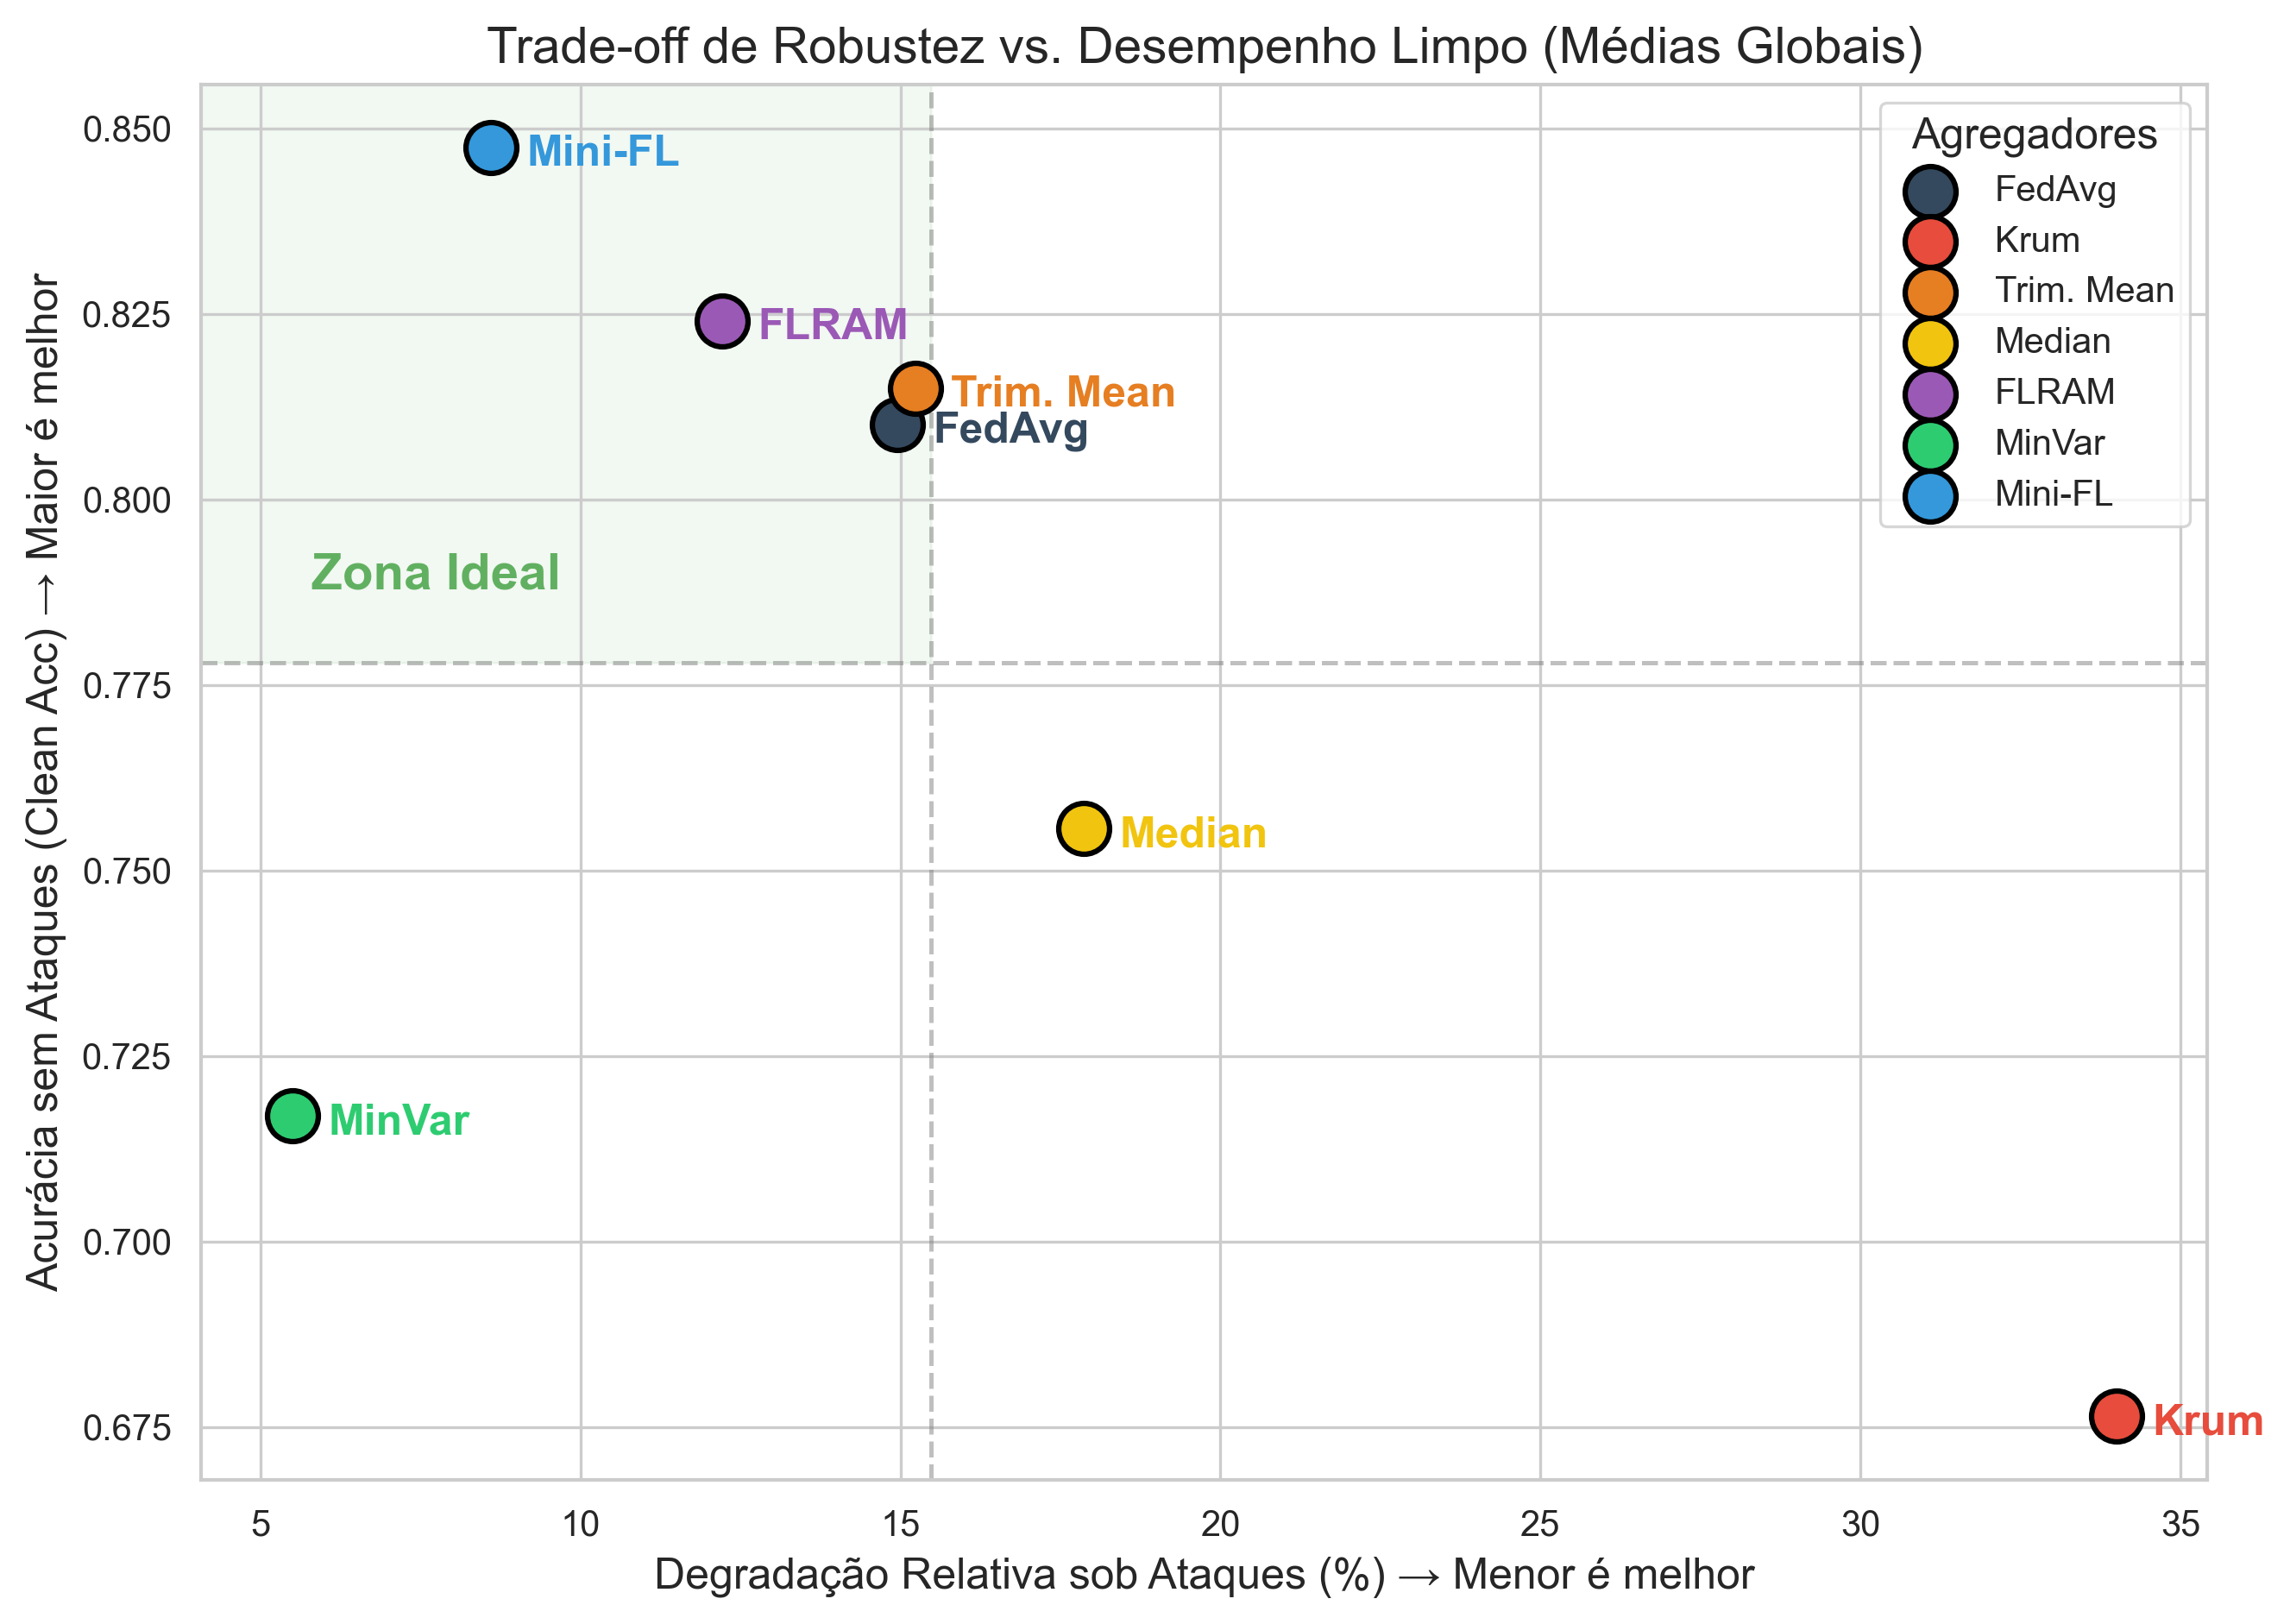
\includegraphics[width=0.9\textwidth]{figuras/fig3_tradeoff_scatter.png}
    \legend{\footnotesize Fonte: elaborado pelo autor.}
\end{figure}

O Mini-FL obteve o primeiro lugar geral, atingindo uma acurácia robusta média de 83,35\% e degradação de apenas 8,6\%. Esse desempenho superior é derivado do mecanismo de agrupamento (\textit{clustering}) que mitiga os efeitos maliciosos de forma granular antes da agregação final.

De forma notável, o algortimo de minimização de variância (MinVar) obteve a menor degradação de todo o conjunto de testes (5,5\%), exibindo uma estabilidade excepcional indepedentemente dos ataques. No entanto, por penalizar variações de forma agnóstica computando limites nas atualizações, o aprendizado basal converge para valores substancialmente menores que agregadores como o Mini-FL.

Os resultados detalhados evidenciam também o decaimento drástico do Krum. Como ilustrado na Figura~\ref{fig:heatmap_mnist}, o Krum sofre uma degradação de modelo em torno de 34\%, com alta susceptibilidade, especialmente no contexto com alta variação onde os defensores acabam sendo removidos devido às distâncias extremas.

\begin{figure}[H]
    \centering
    \caption{Média de degradação relativa (\%) por agregador e tipo de ataque no MNIST}
    \label{fig:heatmap_mnist}
    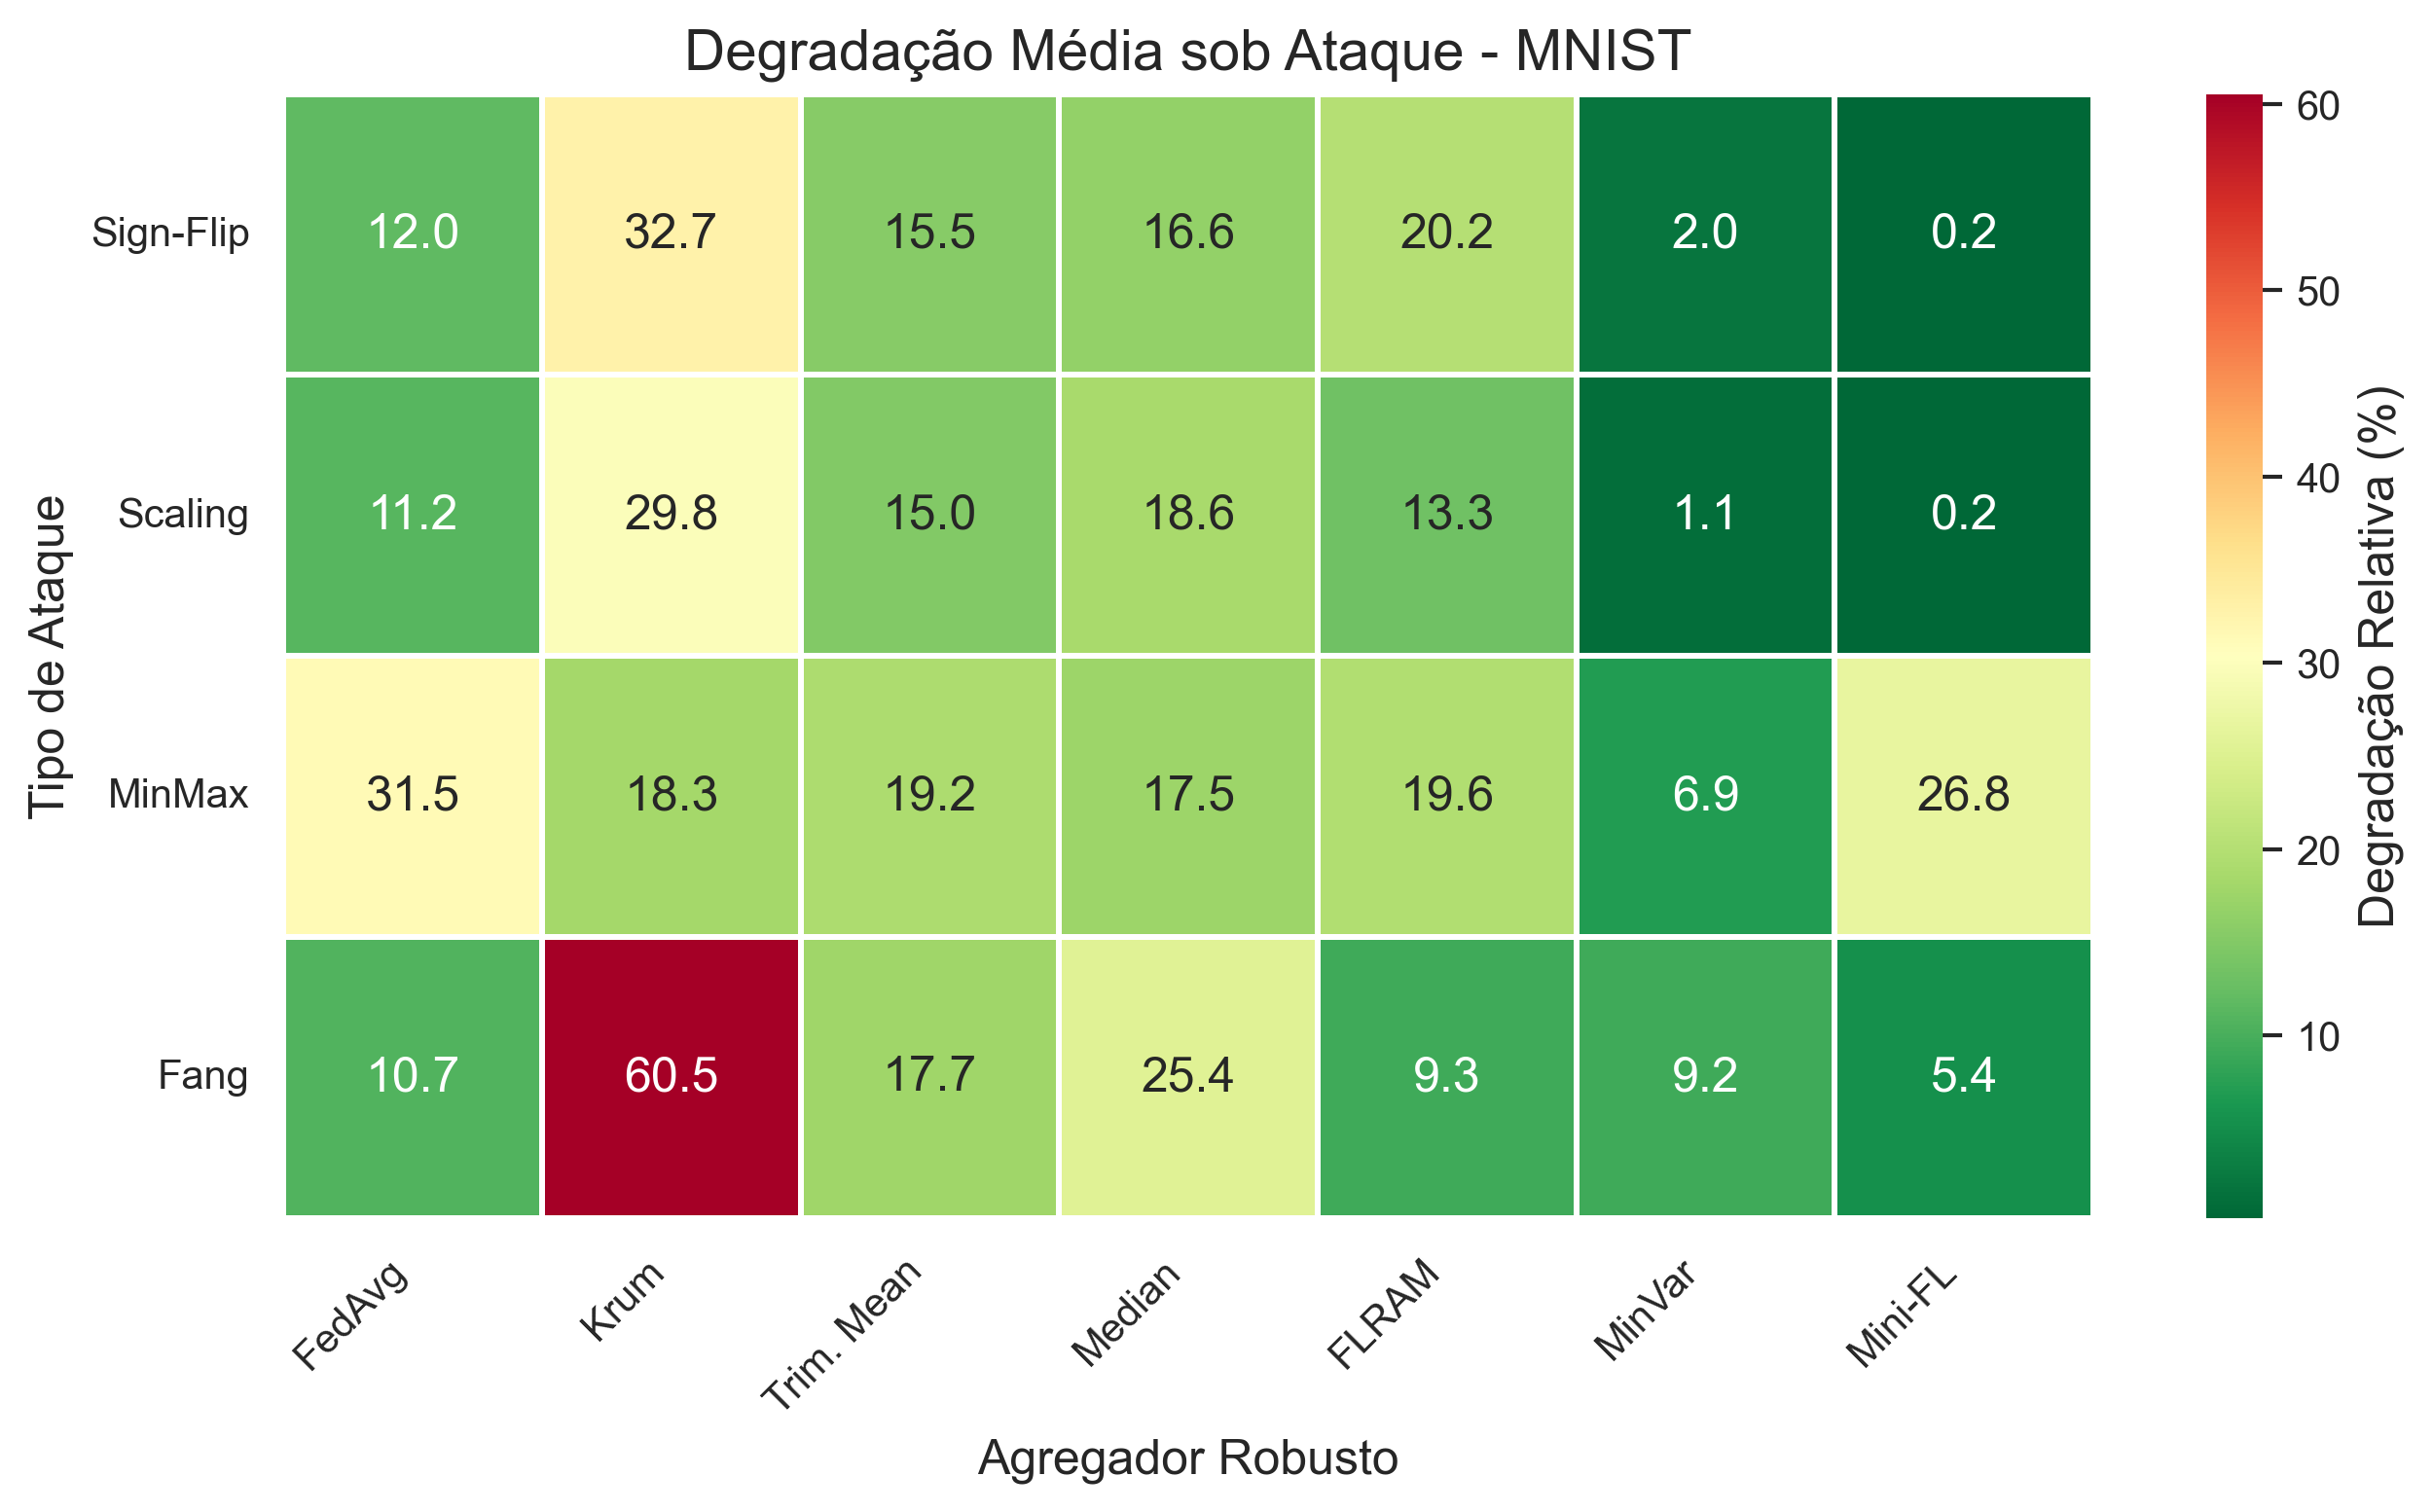
\includegraphics[width=0.9\textwidth]{figuras/fig4_heatmap_degradacao_mnist.png}
    \legend{\footnotesize Fonte: elaborado pelo autor.}
\end{figure}

\section{Comportamento Temporal e Convergência}
\label{sec:res-learning-curves}

Para investigar a dinâmica do aprendizado, as curvas de acurácia por rodada foram observadas em cenários desafiadores. A Figura~\ref{fig:learning_curve_sigflip} apresenta um caso severo: ataque de inversão de sinal (\textit{Sign-Flip}) em um cenário com $40\%$ dos clientes maliciosos e heterogeneidade moderada ($\alpha=0.5$).

\begin{figure}[H]
    \centering
    \caption{Curva de aprendizado sob ataque Sign-Flip ($f_{mal}=0.40$, $\alpha=0.5$) - MNIST}
    \label{fig:learning_curve_sigflip}
    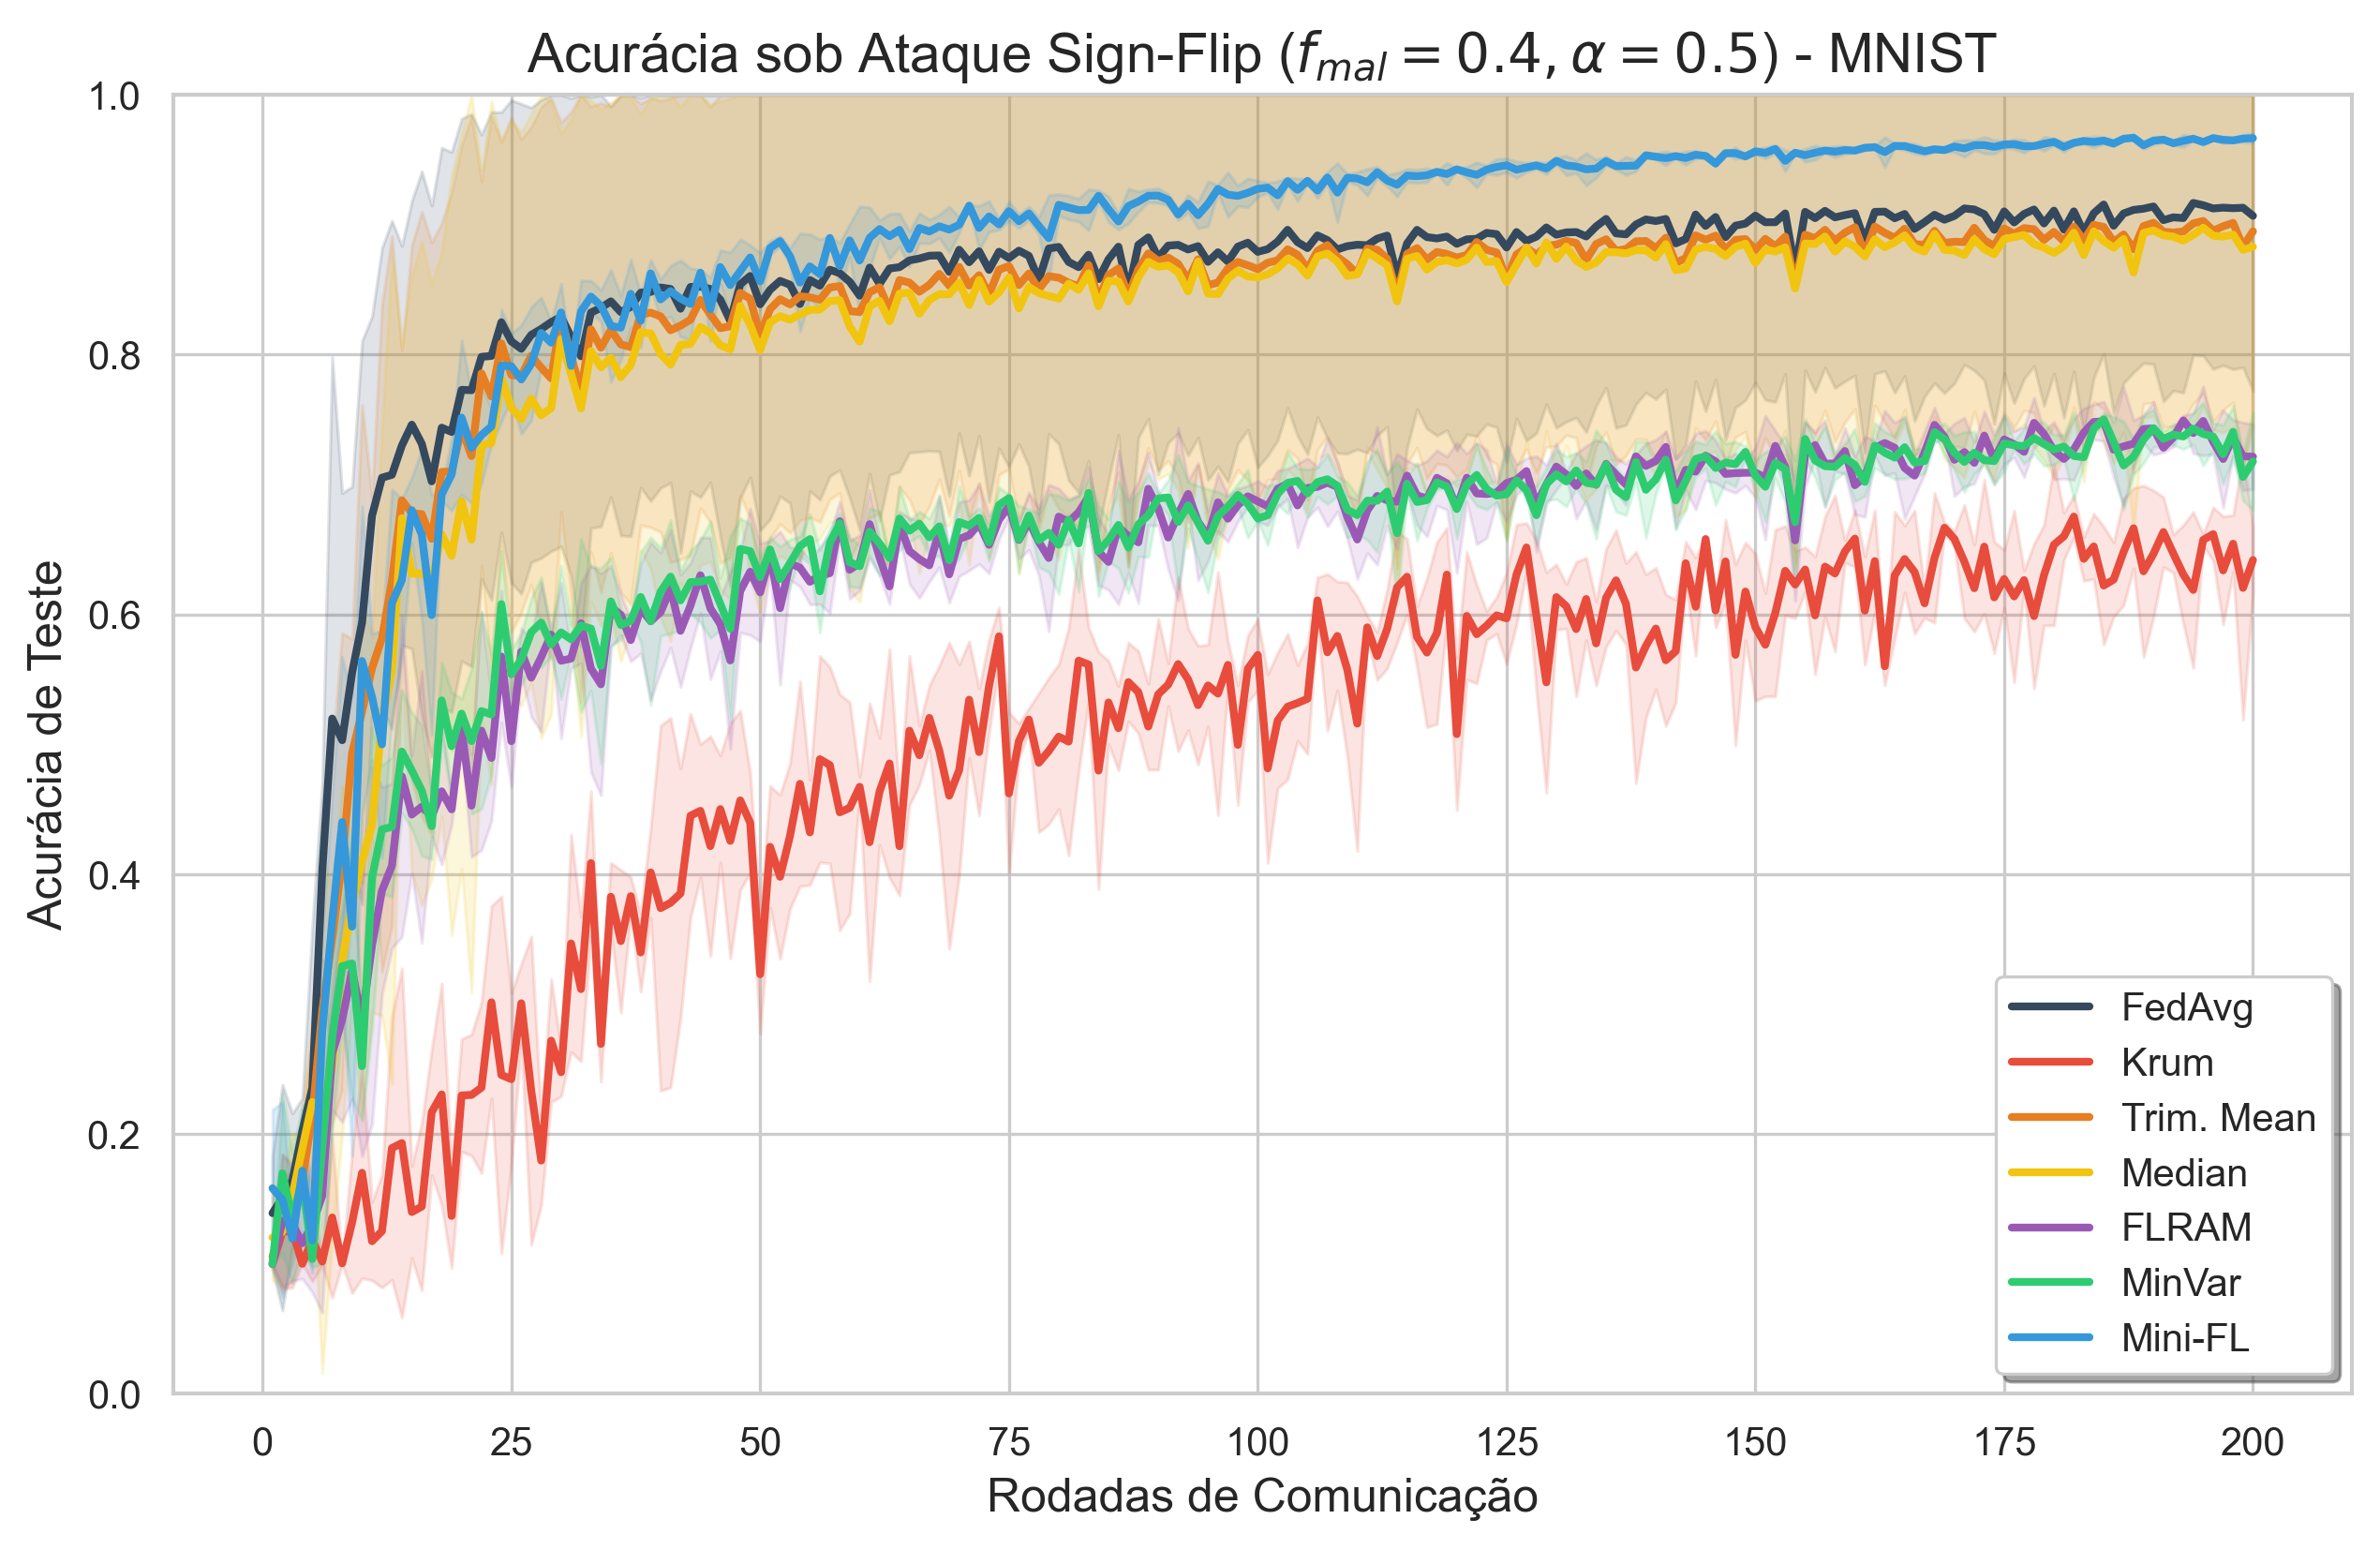
\includegraphics[width=0.9\textwidth]{figuras/fig1_learning_curve_mnist_sign_flip_mf0.4.png}
    \legend{\footnotesize Fonte: elaborado pelo autor.}
\end{figure}

A curva demonstra que, neste nível, métodos como FedAvg não conseguem se recuperar do choque dos gradientes invertidos. Por outro lado, o Trimmed Mean e o FLRAM filtram o ataque de maneira rápida, sendo que o FLRAM apresenta variações estatísticas ($\sigma_{est}$) levemente superiores em regime de convergência, mas alcança maior patamar final.

Em termos de métrica padronizada de rodadas até a convergência (Tabela~\ref{tab:ranking_global}), notou-se que o ganho de robustez nem sempre incorre em um alto atraso de aprendizado. O Mini-FL obteve convergência inicial ao redor da rodada 103, equivalente ou ligeiramente mais precoce que o FedAvg limpo, graças não só à não interferência do ataque mas a um agrupamento mais sinérgico das contribuições \gls{noniid}.

\section{Acurácia por Tipos de Ataques e Domínios Complexos (Fashion-MNIST)}
\label{sec:res-fashion}

Para inferir a relevância dos efeitos encontrados perante uma mudança de domínio de dados e complexidade visual, análises análogas limitadas a ataques direcionáveis foram reproduzidas no Fashion-MNIST.

A Tabela~\ref{tab:wilcoxon} atesta a significância das vantagens de método perante o \textit{baseline} vulnerável (FedAvg).

\begin{table}[H]
\centering
\caption{Testes de Wilcoxon: comparação de cada agregador vs.~FedAvg (baseline)}
\label{tab:wilcoxon}
\footnotesize
\setlength{\tabcolsep}{3pt}
\begin{tabular}{@{}llcccc@{}}
\toprule
\textbf{Dataset} & \textbf{Comparação} & \textbf{Dir.} & \textbf{$p$} & \textbf{$r$} & \textbf{Sig.} \\
\midrule
MNIST & Krum vs.~FedAvg & <FedAvg & 0.0000 & 0.634 & \checkmark \\
MNIST & Trim. Mean vs.~FedAvg & >FedAvg & 0.0206 & 0.273 & \checkmark \\
MNIST & Median vs.~FedAvg & <FedAvg & 0.0007 & 0.400 & \checkmark \\
MNIST & FLRAM vs.~FedAvg & >FedAvg & 0.5614 & 0.068 &  \\
MNIST & MinVar vs.~FedAvg & <FedAvg & 0.0017 & 0.370 & \checkmark \\
MNIST & Mini-FL vs.~FedAvg & >FedAvg & 0.0020 & 0.364 & \checkmark \\
Fashion & Krum vs.~FedAvg & <FedAvg & 0.0000 & 1.081 & \checkmark \\
Fashion & Trim. Mean vs.~FedAvg & <FedAvg & 0.0005 & 0.712 & \checkmark \\
Fashion & Median vs.~FedAvg & <FedAvg & 0.0000 & 1.081 & \checkmark \\
Fashion & FLRAM vs.~FedAvg & >FedAvg & 0.9218 & 0.020 &  \\
Fashion & MinVar vs.~FedAvg & <FedAvg & 0.0646 & 0.377 &  \\
Fashion & Mini-FL vs.~FedAvg & <FedAvg & 0.0032 & 0.601 & \checkmark \\
\bottomrule
\end{tabular}
\legend{\footnotesize Wilcoxon signed-rank, $\alpha=0.05$. $r = |Z|/\sqrt{N}$: tamanho de efeito (>0.1 pequeno, >0.3 médio, >0.5 grande). \checkmark: significativo. Fonte: elaborado pelo autor.}
\end{table}

A Figura~\ref{fig:bar_fashion} destrincha o retorno da acurácia sob diferentes tipos de ameaças no ambiente do Fashion-MNIST. A correlação de Spearman de rankings calculados utilizando ambos domínios (Tabela~\ref{tab:spearman_ranking} - Apêndices) revelou congruência forte ($\rho=0,786$, $p=0,036$). Assim sendo, agregadores como FLRAM e Mini-FL ratificam sua escalabilidade e robustez genérica fora de premissas estritas ou hiper-simplificadas de formato de dados (\textit{data agnostic}).

\begin{figure}[H]
    \centering
    \caption{Comparativo da Acurácia Robusta em presença dos ataques executados para o domínio Fashion-MNIST}
    \label{fig:bar_fashion}
    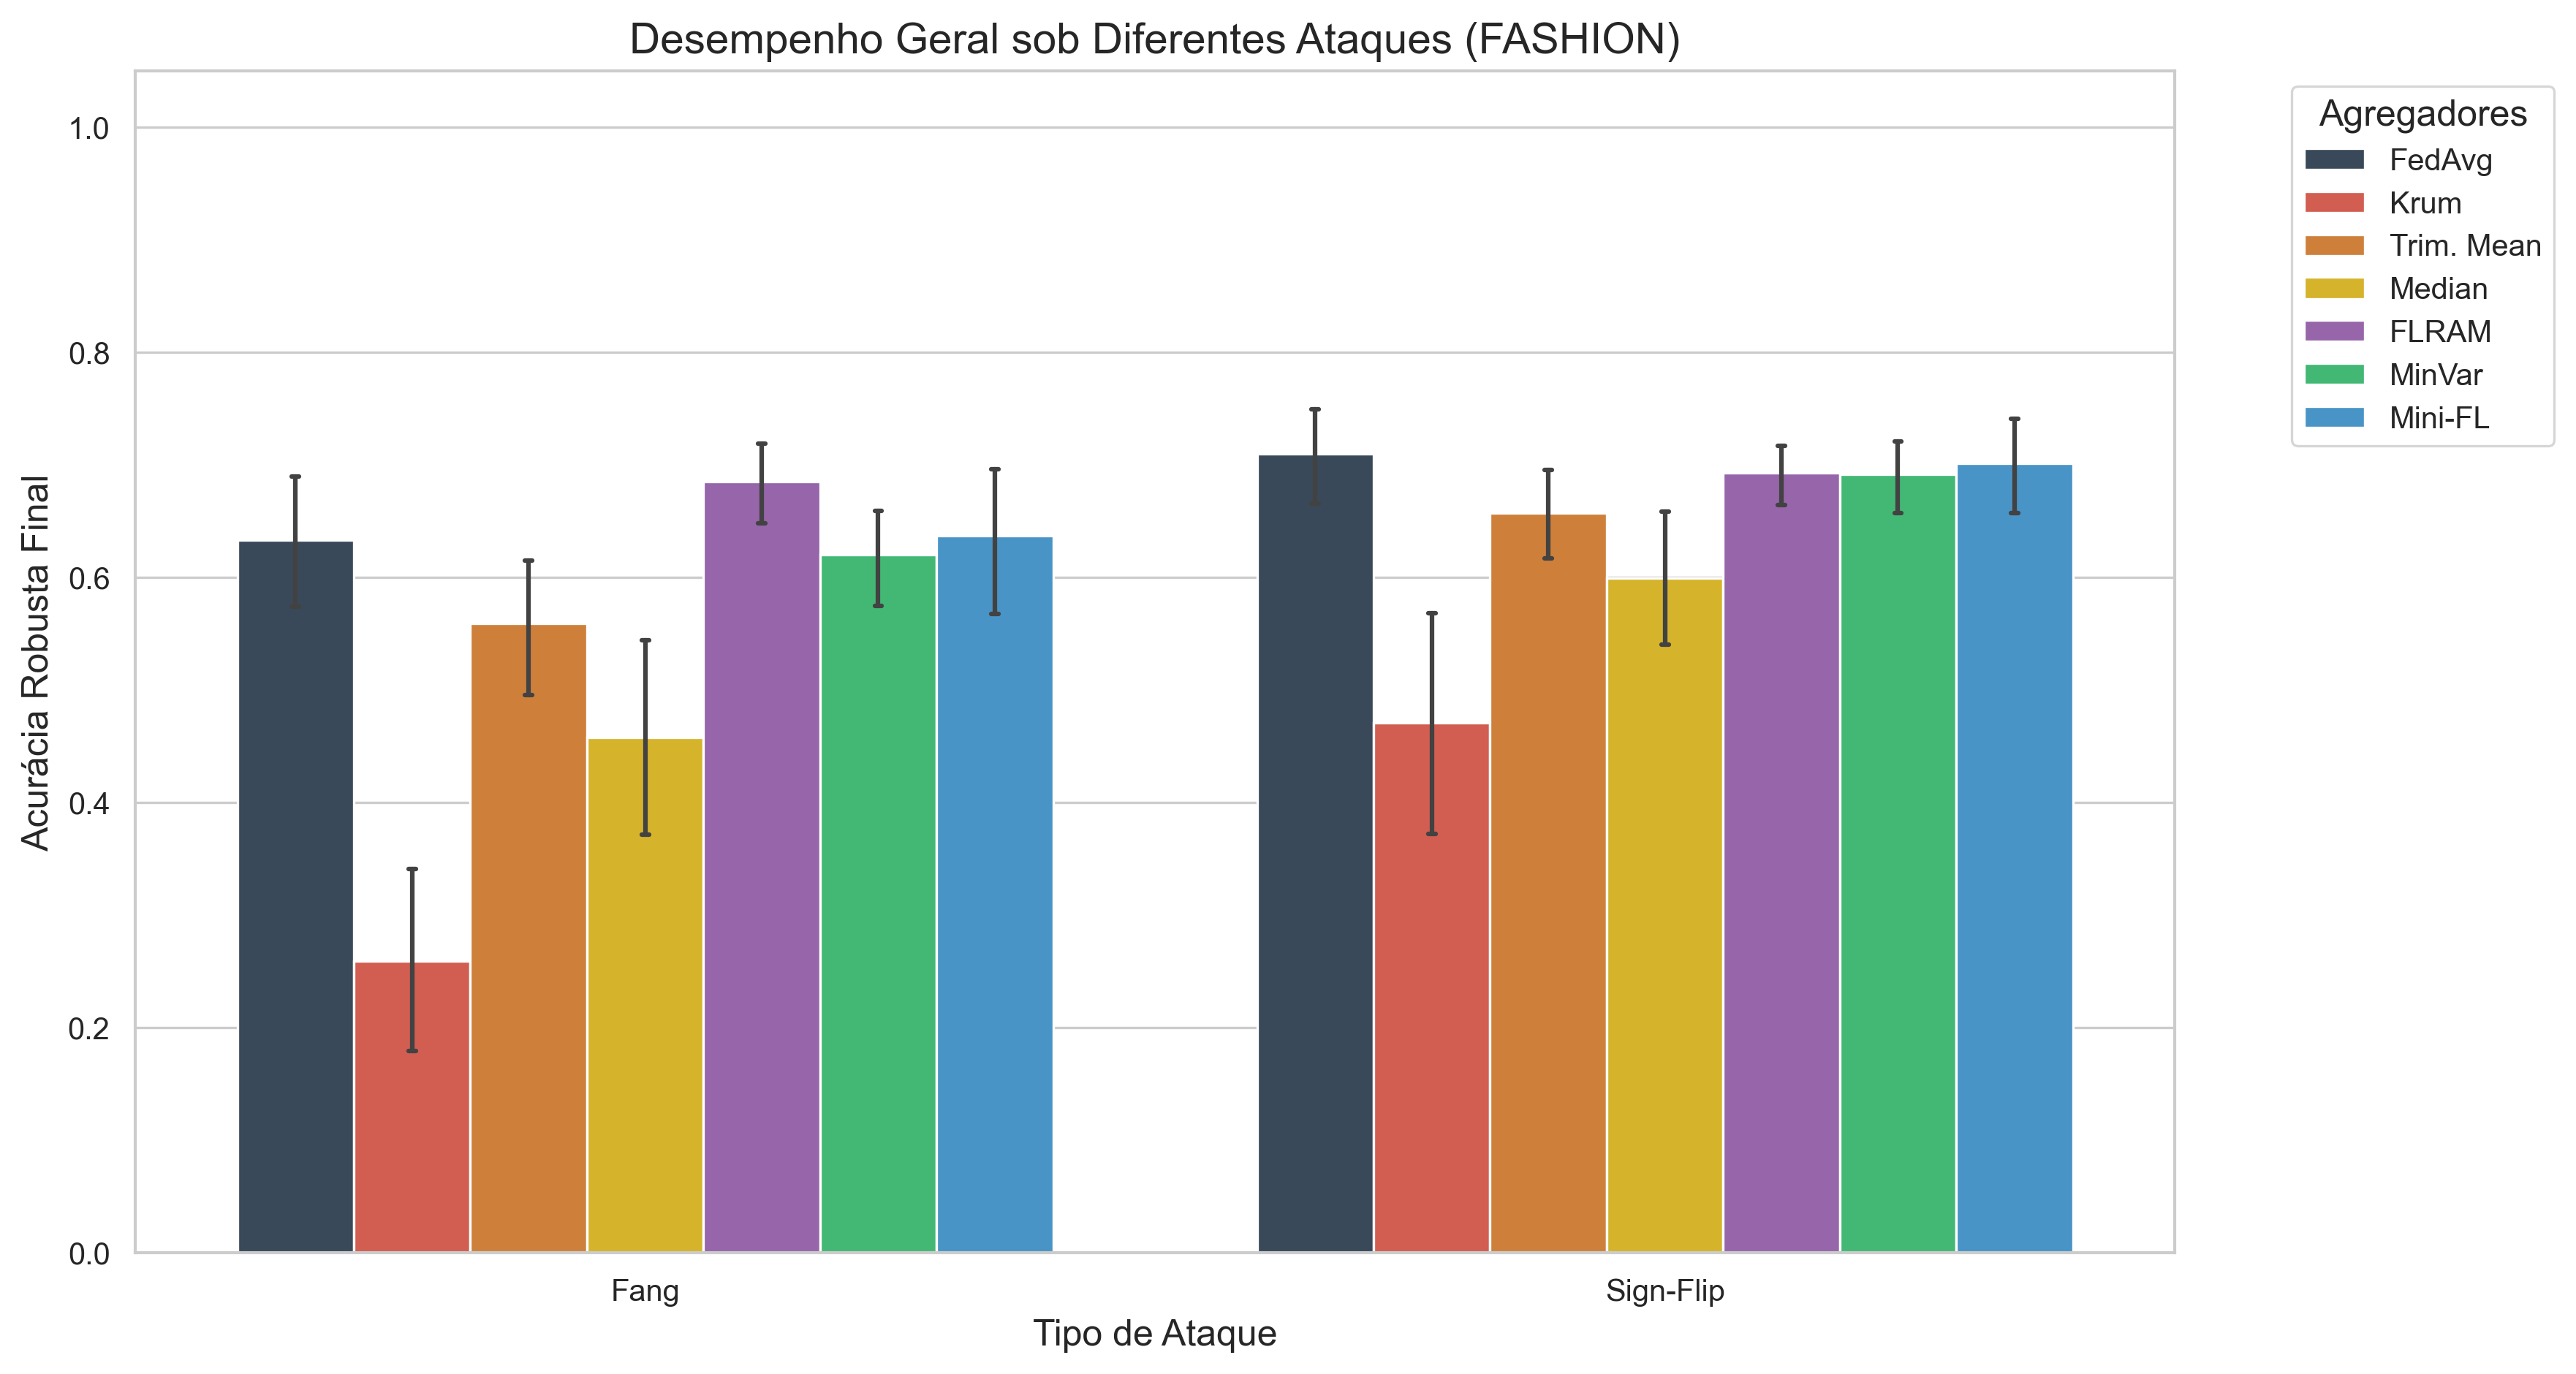
\includegraphics[width=1.0\textwidth]{figuras/fig2_barras_acc_fashion.png}
    \legend{\footnotesize Fonte: elaborado pelo autor.}
\end{figure}

\section{Efeito de Fatores e Intensidades}
\label{sec:res-ablacao}

O aumento quantitativo do número de clientes maliciosos no pool global em cada rodada de agregação impacta diretamente a sobrevivência do modelo (Tabela~\ref{tab:efeito_fmal} do Apêndice). Avaliando a transição da parcela $f_{mal}=0.20$ para $0.40$ – limiar muito perto do teto de tolerância da maioria dos defensores modernos como o método dos Quartis –, observou-se uma queda percentual de $11$-$18$ pontos para a Mediana em certas \textit{seeds}, enquanto o Trimmed Mean demonstrou perda quase nula contra anomalias escalares extremas (\textit{Scaling Attack}). No entanto, o Trimmed Mean sofre quando se eleva a presença e variabilidade Non-IID ao limite da exclusão indiscriminada dos gradientes saudáveis.

\section{Síntese da Avaliação Experimental}
\label{sec:res-sintese}

Os 777 experimentos conduzidos permitem evidenciar as seguintes constatações na implementação da segurança dos ecossistemas de FL (\gls{fl}) \cite{Liang2023,Mothukuri2021}:

\begin{enumerate}
    \item Defesas pautadas pela remoção completa com base em distâncias diretas, exemplificadas pelo \textbf{Krum}, são severamente prejudicadas por partições fortemente estatisticamente díspares, tendendo a eleger modelos falhos devido a similaridade vetorial artificial de ataques como o \textit{MinMax}.
    \item \textbf{MinVar} representa uma escolha arquitetônica garantidora do topo de estabilidade. Caso haja margem para abdicar de 10--15\% da performance teto da rede neural para evitar interrupções ou flutuações violentas de perda (\textit{loss variance}), é a recomendação imediata.
    \item  A detecção inteligente do \textbf{FLRAM} ou o particionamento latente do \textbf{Mini-FL} configuram o moderno padrão ouro testado, visto que são capazes de contornar a distorção \textit{byzantine} (adversarial) e absorver positivamente os benefícios da heterogeneidade em direção e intensidade durante treinos iterativos.
\end{enumerate}


\chapter*{Apêndices}
\addcontentsline{toc}{chapter}{Apêndices}

% --- T1_clean_acc_mnist.tex ---
\begin{table}[H]
\centering
\caption{Acurácia final (Acc$_{final}$) sem adversários — MNIST (média ± dp, $n=3$ seeds)}
\label{tab:clean_acc_mnist}
\footnotesize
\setlength{\tabcolsep}{3pt}
\begin{tabular}{@{}lccc@{}}
\toprule
\textbf{Agregador} & \textbf{α=0.1} & \textbf{α=0.5} & \textbf{α=1.0} \\
\midrule
FedAvg & 0.981 ± 0.003 & 0.688 ± 0.417 & 0.978 ± 0.006 \\
Krum & 0.805 ± 0.023 & 0.926 ± 0.019 & 0.962 ± 0.013 \\
Trim. Mean & 0.971 ± 0.001 & 0.972 ± 0.010 & 0.976 ± 0.008 \\
Median & 0.945 ± 0.003 & 0.948 ± 0.005 & 0.974 ± 0.010 \\
FLRAM & 0.959 ± 0.005 & 0.970 ± 0.008 & 0.976 ± 0.006 \\
MinVar & 0.752 ± 0.137 & 0.747 ± 0.010 & 0.743 ± 0.007 \\
Mini-FL & 0.966 ± 0.010 & 0.965 ± 0.002 & 0.966 ± 0.001 \\
\bottomrule
\end{tabular}
\legend{\footnotesize Fonte: elaborado pelo autor.}
\end{table}
% --- T1_clean_acc_fashion.tex ---
\begin{table}[H]
\centering
\caption{Acurácia final (Acc$_{final}$) sem adversários — Fashion-MNIST (média ± dp, $n=3$ seeds)}
\label{tab:clean_acc_fashion}
\footnotesize
\setlength{\tabcolsep}{3pt}
\begin{tabular}{@{}lcc@{}}
\toprule
\textbf{Agregador} & \textbf{α=0.1} & \textbf{α=0.5} \\
\midrule
FedAvg & 0.720 ± 0.011 & 0.773 ± 0.005 \\
Krum & 0.345 ± 0.001 & 0.674 ± 0.031 \\
Trim. Mean & 0.618 ± 0.024 & 0.736 ± 0.013 \\
Median & 0.474 ± 0.017 & 0.720 ± 0.022 \\
FLRAM & 0.646 ± 0.039 & 0.747 ± 0.021 \\
MinVar & 0.656 ± 0.010 & 0.747 ± 0.010 \\
Mini-FL & 0.714 ± 0.014 & 0.760 ± 0.009 \\
\bottomrule
\end{tabular}
\legend{\footnotesize Fonte: elaborado pelo autor.}
\end{table}
% --- T4_degradacao_mnist.tex ---
\begin{table}[H]
\centering
\caption{Degradação relativa (\%) por agregador e ataque — MNIST}
\label{tab:degradacao_mnist}
\footnotesize
\setlength{\tabcolsep}{3pt}
\begin{tabular}{@{}lcccc@{}}
\toprule
\textbf{Agregador} & \textbf{Fang} & \textbf{MinMax} & \textbf{Scaling} & \textbf{Sign-Flip} \\
\midrule
FedAvg & 10.7 ± 12.0 & 31.5 ± 22.7 & 11.2 ± 13.7 & 12.0 ± 14.2 \\
Krum & 60.5 ± 31.8 & 18.3 ± 16.7 & 29.8 ± 25.3 & 32.7 ± 23.0 \\
Trim. Mean & 17.7 ± 14.9 & 19.2 ± 12.1 & 15.0 ± 13.5 & 15.5 ± 14.0 \\
Median & 25.4 ± 23.8 & 17.5 ± 15.1 & 18.6 ± 15.5 & 16.6 ± 16.6 \\
FLRAM & 9.3 ± 11.3 & 19.6 ± 11.7 & 13.3 ± 14.0 & 20.2 ± 11.6 \\
MinVar & 9.2 ± 9.8 & \textbf{6.9 ± 12.0} & 1.1 ± 3.1 & 2.0 ± 3.6 \\
Mini-FL & \textbf{5.4 ± 7.2} & 26.8 ± 26.9 & \textbf{0.2 ± 0.5} & \textbf{0.2 ± 0.5} \\
\bottomrule
\end{tabular}
\legend{\footnotesize Degradação ($\delta\%$) = (Acc$_{limpa}$ - Acc$_{rob}$) / Acc$_{limpa}$ × 100. Negrito: menor degradação por ataque. Fonte: elaborado pelo autor.}
\end{table}
% --- T5_degradacao_fashion.tex ---
\begin{table}[H]
\centering
\caption{Degradação relativa (\%) por agregador e ataque — Fashion-MNIST}
\label{tab:degradacao_fashion}
\footnotesize
\setlength{\tabcolsep}{3pt}
\begin{tabular}{@{}lcc@{}}
\toprule
\textbf{Agregador} & \textbf{Fang} & \textbf{Sign-Flip} \\
\midrule
FedAvg & 15.6 ± 13.0 & 5.7 ± 7.6 \\
Krum & 46.0 ± 23.4 & 10.9 ± 12.8 \\
Trim. Mean & 16.3 ± 14.8 & 4.1 ± 4.4 \\
Median & 21.8 ± 21.9 & 2.9 ± 4.0 \\
FLRAM & \textbf{3.3 ± 6.5} & 3.0 ± 3.5 \\
MinVar & 11.4 ± 8.8 & \textbf{2.9 ± 4.1} \\
Mini-FL & 14.2 ± 13.4 & 5.7 ± 8.1 \\
\bottomrule
\end{tabular}
\legend{\footnotesize Degradação ($\delta\%$) = (Acc$_{limpa}$ - Acc$_{rob}$) / Acc$_{limpa}$ × 100. Negrito: menor degradação por ataque. Fonte: elaborado pelo autor.}
\end{table}
% --- T6_convergencia_mnist.tex ---
\begin{table}[H]
\centering
\caption{Rodadas para convergência por agregador e heterogeneidade — MNIST}
\label{tab:convergencia_mnist}
\footnotesize
\setlength{\tabcolsep}{3pt}
\begin{tabular}{@{}lccc@{}}
\toprule
\textbf{Agregador} & \textbf{α=0.1} & \textbf{α=0.5} & \textbf{α=1.0} \\
\midrule
FedAvg & 86.9 ± 49.3 & 102.4 ± 38.2 & 92.5 ± 40.2 \\
Krum & 150.9 ± 57.9 & 118.5 ± 36.0 & 95.7 ± 34.8 \\
Trim. Mean & 116.9 ± 36.1 & 98.7 ± 26.5 & 84.8 ± 26.0 \\
Median & 129.2 ± 29.2 & 107.5 ± 25.6 & 85.4 ± 25.9 \\
FLRAM & 111.4 ± 28.6 & 103.6 ± 29.7 & 85.7 ± 24.5 \\
MinVar & 126.0 ± 28.8 & 116.7 ± 17.0 & 99.3 ± 15.3 \\
Mini-FL & 95.1 ± 38.3 & 97.7 ± 27.9 & 88.2 ± 26.0 \\
\bottomrule
\end{tabular}
\legend{\footnotesize Rodadas até Acc $\geq$ 95\% do pico. Média ± dp sobre todos os cenários de ataque. Fonte: elaborado pelo autor.}
\end{table}
% --- T7_estabilidade_mnist.tex ---
\begin{table}[H]
\centering
\caption{Estabilidade (σ) nas rodadas 150--200 por agregador e ataque — MNIST}
\label{tab:estabilidade_mnist}
\footnotesize
\setlength{\tabcolsep}{3pt}
\begin{tabular}{@{}lcccc@{}}
\toprule
\textbf{Agregador} & \textbf{Fang} & \textbf{MinMax} & \textbf{Scaling} & \textbf{Sign-Flip} \\
\midrule
FedAvg & 0.0172 & 0.0594 & 0.0158 & 0.0154 \\
Krum & 0.0350 & 0.0495 & 0.0417 & 0.0450 \\
Trim. Mean & 0.0210 & 0.0270 & 0.0162 & 0.0158 \\
Median & 0.0318 & 0.0259 & 0.0233 & 0.0181 \\
FLRAM & 0.0189 & 0.0415 & 0.0192 & 0.0289 \\
MinVar & 0.0273 & 0.0379 & 0.0142 & 0.0196 \\
Mini-FL & 0.0160 & 0.0400 & 0.0062 & 0.0062 \\
\bottomrule
\end{tabular}
\legend{\footnotesize σ = desvio padrão da acurácia nas rodadas 150--200 (proxy de estabilidade pós-convergência). Fonte: elaborado pelo autor.}
\end{table}
% --- T10_f1_mnist.tex ---
\begin{table}[H]
\centering
\caption{F1-Score macro por agregador e ataque — MNIST (média ± dp)}
\label{tab:f1_mnist}
\footnotesize
\setlength{\tabcolsep}{3pt}
\begin{tabular}{@{}lcccc@{}}
\toprule
\textbf{Agregador} & \textbf{Fang} & \textbf{MinMax} & \textbf{Scaling} & \textbf{Sign-Flip} \\
\midrule
FedAvg & 0.827 ± 0.145 & 0.615 ± 0.220 & 0.849 ± 0.147 & 0.843 ± 0.151 \\
Krum & 0.295 ± 0.335 & 0.713 ± 0.199 & 0.605 ± 0.296 & 0.571 ± 0.263 \\
Trim. Mean & 0.782 ± 0.164 & 0.768 ± 0.131 & 0.814 ± 0.148 & 0.809 ± 0.155 \\
Median & 0.686 ± 0.266 & \textbf{0.770 ± 0.163} & 0.759 ± 0.172 & 0.784 ± 0.185 \\
FLRAM & 0.871 ± 0.126 & 0.757 ± 0.139 & 0.830 ± 0.151 & 0.758 ± 0.127 \\
MinVar & 0.680 ± 0.144 & 0.702 ± 0.135 & 0.836 ± 0.138 & 0.759 ± 0.134 \\
Mini-FL & \textbf{0.908 ± 0.082} & 0.657 ± 0.307 & \textbf{0.966 ± 0.005} & \textbf{0.966 ± 0.005} \\
\bottomrule
\end{tabular}
\legend{\footnotesize Negrito: melhor por coluna. Fonte: elaborado pelo autor.}
\end{table}
% --- T11_spearman_ranking.tex ---
\begin{table}[H]
\centering
\caption{Ranking de robustez: acurácia média sob ataque (MNIST vs.~Fashion-MNIST)}
\label{tab:spearman_ranking}
\footnotesize
\setlength{\tabcolsep}{3pt}
\begin{tabular}{@{}lccc@{}}
\toprule
\textbf{Agregador} & \textbf{MNIST (Acc$_{rob}$)} & \textbf{Fashion (Acc$_{rob}$)} & \textbf{Rank MNIST} \\
\midrule
Mini-FL & 0.8882 & 0.6694 & 1 \\
FLRAM & 0.8183 & 0.6887 & 2 \\
Trim. Mean & 0.8091 & 0.6028 & 3 \\
FedAvg & 0.8003 & 0.6673 & 4 \\
Median & 0.7707 & 0.5209 & 5 \\
MinVar & 0.7638 & 0.6533 & 6 \\
Krum & 0.5908 & 0.3534 & 7 \\
\midrule
\multicolumn{4}{l}{Correlação de Spearman: $\rho = 0.786$, $p = 0.036$} \\
\bottomrule
\end{tabular}
\legend{\footnotesize $\rho$ mede a consistência do ranking entre os dois datasets. Fonte: elaborado pelo autor.}
\end{table}
% --- T12_efeito_fmal.tex ---
\begin{table}[H]
\centering
\caption{Efeito da fração de adversários ($f_{mal}$) na acurácia robusta — MNIST}
\label{tab:efeito_fmal}
\footnotesize
\setlength{\tabcolsep}{3pt}
\begin{tabular}{@{}lccc@{}}
\toprule
\textbf{Agregador} & \textbf{$f_{mal}=0.2$} & \textbf{$f_{mal}=0.4$} & \textbf{Δ (p.p.)} \\
\midrule
FedAvg & 0.7687 & 0.8319 & +6.32 \\
Krum & 0.6014 & 0.5802 & -2.11 \\
Trim. Mean & 0.7564 & 0.8618 & +10.54 \\
Median & 0.7257 & 0.8158 & +9.01 \\
FLRAM & 0.7896 & 0.8470 & +5.73 \\
MinVar & 0.7207 & 0.8069 & +8.61 \\
Mini-FL & 0.9438 & 0.8326 & -11.11 \\
\bottomrule
\end{tabular}
\legend{\footnotesize Δ = Acc($f_{mal}$=0.4) $-$ Acc($f_{mal}$=0.2) em pontos percentuais. Médias sobre todos os ataques e valores de α. Fonte: elaborado pelo autor.}
\end{table}
% --- T2_robust_acc_mnist.tex ---
\begin{table}[H]
\centering
\caption{Acurácia robusta (Acc$_{rob}$) por agregador e ataque — MNIST (média sobre $\alpha$ e $f_{mal}$; $n \geq 3$)}
\label{tab:robust_acc_mnist}
\footnotesize
\setlength{\tabcolsep}{3pt}
\begin{tabular}{@{}lcccc@{}}
\toprule
\textbf{Agregador} & \textbf{Fang} & \textbf{MinMax} & \textbf{Scaling} & \textbf{Sign-Flip} \\
\midrule
FedAvg & 0.842 ± 0.127 & 0.648 ± 0.199 & 0.858 ± 0.133 & 0.852 ± 0.138 \\
Krum & 0.363 ± 0.307 & 0.739 ± 0.173 & 0.645 ± 0.261 & 0.616 ± 0.234 \\
Trim. Mean & 0.800 ± 0.145 & 0.786 ± 0.118 & 0.827 ± 0.132 & 0.823 ± 0.139 \\
Median & 0.714 ± 0.232 & \textbf{0.789 ± 0.147} & 0.779 ± 0.152 & 0.801 ± 0.164 \\
FLRAM & 0.880 ± 0.112 & 0.779 ± 0.114 & 0.841 ± 0.137 & 0.773 ± 0.115 \\
MinVar & 0.705 ± 0.128 & 0.730 ± 0.116 & 0.846 ± 0.125 & 0.774 ± 0.121 \\
Mini-FL & \textbf{0.914 ± 0.067} & 0.707 ± 0.259 & \textbf{0.966 ± 0.005} & \textbf{0.966 ± 0.005} \\
\bottomrule
\end{tabular}
\legend{\footnotesize Valores em média ± dp ($n \geq 3$). Negrito: melhor por coluna. Fonte: elaborado pelo autor.}
\end{table}
% --- T3_robust_acc_fashion.tex ---
\begin{table}[H]
\centering
\caption{Acurácia robusta (Acc$_{rob}$) por agregador e ataque — Fashion-MNIST (média sobre $\alpha$ e $f_{mal}$)}
\label{tab:robust_acc_fashion}
\footnotesize
\setlength{\tabcolsep}{3pt}
\begin{tabular}{@{}lcc@{}}
\toprule
\textbf{Agregador} & \textbf{Fang} & \textbf{Sign-Flip} \\
\midrule
FedAvg & 0.633 ± 0.114 & \textbf{0.710 ± 0.074} \\
Krum & 0.259 ± 0.162 & 0.471 ± 0.186 \\
Trim. Mean & 0.559 ± 0.124 & 0.657 ± 0.070 \\
Median & 0.458 ± 0.176 & 0.600 ± 0.104 \\
FLRAM & \textbf{0.685 ± 0.068} & 0.693 ± 0.048 \\
MinVar & 0.620 ± 0.084 & 0.692 ± 0.056 \\
Mini-FL & 0.637 ± 0.114 & 0.702 ± 0.075 \\
\bottomrule
\end{tabular}
\legend{\footnotesize Valores em média ± dp ($n \geq 3$). Negrito: melhor por coluna. Fonte: elaborado pelo autor.}
\end{table}

\chapter*{Apêndices}
\addcontentsline{toc}{chapter}{Apêndices}


